\documentclass[11pt,a4paper]{article}

\usepackage[T1]{fontenc}
\usepackage[utf8]{inputenc}
\usepackage{mathptmx}
\usepackage{courier}
\usepackage[margin=2.5cm]{geometry}
\usepackage{amsmath}
\usepackage{booktabs}
\usepackage{graphicx}
\usepackage{xcolor}
\usepackage[numbers,sort&compress]{natbib}
\usepackage{xurl}
\usepackage[hidelinks]{hyperref}
\hypersetup{pdftitle={Pretrained Backbones, Calibration and Referral for Fracture Detection on FracAtlas},pdfauthor={Muzammal Hussain}}
\usepackage{caption}
\captionsetup{font=small,labelfont=bf}

\newcommand{\code}[1]{\texttt{#1}}
\setlength{\emergencystretch}{3em}

\title{\textbf{Pretrained Backbones, Calibration and Referral\\for Fracture Detection on FracAtlas:\\A Three-Seed Comparison of a Small CNN, ConvNeXt, DINOv2 and YOLO}}
\author{Muzammal Hussain\\
\small Independent researcher, Glasgow, United Kingdom\\
\small \href{mailto:muzammal@masmatixinnovations.co.uk}{muzammal@masmatixinnovations.co.uk}\\
\small ORCID: \href{https://orcid.org/0009-0001-2570-5686}{0009-0001-2570-5686}}
\date{\small November 2026}

\begin{document}
\maketitle

\begin{abstract}
\noindent
FracAtlas is the largest openly licensed set of musculoskeletal X-rays with expert fracture labels and boxes, but it
has no classification baseline or fixed test split, and later results on it are single-run accuracies on splits of
their own. We fix a 70/15/15 split stratified by label and body region (614 test images, 109 fractured) and train four
classifiers with three seeds each: a small CNN from scratch, ImageNet-pretrained ConvNeXt-Tiny, and DINOv2 ViT-S/14 as
a frozen probe or fine-tuned; a YOLO11s detector is trained on the boxes. Thresholds and temperatures are fitted on
validation data only, with 1,000-sample bootstrap intervals on test. ConvNeXt-Tiny is the strongest and most stable
model (AUROC $0.922 \pm 0.006$ over seeds; seed ensemble 0.928 [0.891, 0.957]), ahead of fine-tuned DINOv2 by
$+0.026$ [$+0.005$, $+0.045$], the frozen probe by $+0.054$ [$+0.026$, $+0.082$] and the small CNN by $+0.118$
[$+0.086$, $+0.151$]. At 90\% specificity it finds 81\% of fractured images, against 44\% for the small CNN.
After temperature scaling ConvNeXt has an expected
calibration error of 0.036 and refers 10\% of images at a confidence cut-off of 0.8 (small CNN: 45\%); referring its
least confident fifth raises accuracy on the rest from 0.906 to 0.961. Leg radiographs are its weak point (AUROC
0.880; 15 of 24 missed fractures). Removing test images that are exact or near copies of training images (perceptual
hash) changes ConvNeXt's AUROC by at most 0.004. The detector ranks images well (AUROC 0.882) but localises moderately (mAP@0.5
0.321). Code, notebooks and weights are released; the models are not for clinical use.
\end{abstract}

\section{Introduction}

Fractures are among the most common reasons for an emergency visit, and a missed fracture on a radiograph delays
treatment. Deep networks trained on large private collections can detect fractures and help clinicians
\citep{lindsey2018fracture}; a meta-analysis of 42 studies found pooled sensitivity and specificity of AI comparable
to clinicians, but judged about half of the studies at high risk of bias \citep{kuo2022fracture}. Much of that work
uses private data, which makes it hard to reproduce. FracAtlas \citep{abedeen2023fracatlas} was released to fill this
gap: 4,083 X-rays of the hand, leg, hip and shoulder from three hospitals in Bangladesh, labelled by two radiologists
and an orthopaedic surgeon, with 922 fracture boxes and masks, under a CC BY 4.0 licence.

The dataset paper validated only detection and segmentation, with YOLOv8 trained on fractured images and evaluated
on a validation subset \citep{abedeen2023fracatlas}. It gives no image-level classification baseline and no fixed
test split. Later work reports accuracy, precision and F1 from a single run on a split of its own, without AUROC or
intervals: for example 90.5\% with attention-based transfer learning \citep{ruhi2024attention} and 96.0\% with a
custom CNN \citep{hassan2025fracture}. With 82\% of images non-fractured, accuracy alone is hard to interpret, and
single runs on different splits say little about how much of a difference between models is due to the seed or the
test sample, and nothing about what a model does when it is unsure. These are the questions a reader needs answered before a model is used to triage images.

\noindent This paper asks four narrow questions:
\begin{enumerate}
\item How much do an ImageNet-pretrained ConvNeXt and a self-supervised DINOv2 backbone gain over a small CNN trained
from scratch on about 2,900 training images, once seed variation and test-sampling uncertainty are reported?
\item Which body regions are hardest?
\item After calibration, how many images must a model refer to a clinician to reach a given sensitivity on the
images it keeps?
\item Does a box detector rank images as well as a classifier when its highest box confidence is used as the image
score?
\end{enumerate}

\noindent The contributions are a fixed, reproducible split and protocol for FracAtlas; a three-seed comparison of
four classifiers with bootstrap intervals and paired differences; per-region results; calibration and
referral (selective prediction) curves with all choices made on validation data; and a released package with code, a
Kaggle notebook, per-seed logits and model weights.

\section{Related work}

\paragraph{Fracture detection.} \citet{lindsey2018fracture} trained a network on 135,409 wrist radiographs annotated
by orthopaedic surgeons and showed that it improved emergency clinicians' reading. MURA \citep{rajpurkar2017mura}
provides 40,561 upper-limb images with normal and abnormal study labels, but without boxes and without separating
fractures from other abnormalities. \citet{kuo2022fracture} pooled 42 studies and found AI sensitivity of about 91\%
on external test sets, similar to clinicians, while noting frequent risk of bias. FracAtlas is smaller than these
collections but is open and carries box and mask annotations \citep{abedeen2023fracatlas}; its authors reported a
YOLOv8s box mAP@0.5 of 0.562 on a validation set of 82 fractured images.

\paragraph{Backbones.} ConvNeXt \citep{liu2022convnext} modernises the residual convolutional network and, in its
ImageNet-22k-pretrained form, is a strong transfer backbone. DINOv2 \citep{oquab2024dinov2} learns general visual
features by self-supervision on 142 million curated natural images and is often used as a frozen feature extractor.
Neither was trained on radiographs, so whether their features transfer to small fracture datasets is an empirical
question.

\paragraph{Calibration and abstention.} Modern networks are often over-confident; temperature scaling fitted on
validation data is a simple fix \citep{guo2017calibration}, and expected calibration error (ECE)
\citep{naeini2015ece} measures the gap between confidence and accuracy. Selective classification
\citep{geifman2017selective} lets a model abstain on its least confident inputs, which in a clinical workflow means
referring them to a human reader. \citet{varoquaux2022failures} list common evaluation failures in medical imaging,
among them single runs, missing intervals and leakage between training and test data; our protocol is designed
around them.

\section{Data and setup}

\paragraph{Data.} We use FracAtlas as released on figshare \citep{abedeen2023fracatlas}; the archive is downloaded at
run time and not redistributed. Its metadata file lists 4,083 images, of which 719 are marked as fractured (the
dataset paper reports 717). Each image is assigned a primary body region from the metadata flags; images flagged with
more than one region form a separate ``multiple'' group. FracAtlas releases no patient identifiers, so the split is
by image: within each combination of label and region, images are shuffled with a fixed seed and divided 70/15/15
into training (2,855 images, 501 fractured), validation (614, 109) and test (614, 109). The test set holds 319 leg
(32 fractured), 192 hand (57), 60 multiple-region (16), 27 hip (2) and 16 shoulder (2) images. Most fractured hip and
shoulder images are also flagged with another region and therefore fall in the multiple-region group; only 10 images
of each are hip-only or shoulder-only fractures. The archive contains a few truncated JPEG files; they
are decoded as far as possible, listed in the run log, and kept.

\paragraph{Classifiers.} Images are converted to grey, letterboxed to a square (aspect ratio kept) and repeated over
three channels with ImageNet normalisation. Table~\ref{tab:setup} lists the four classifiers. The small CNN has five
blocks of two $3\times3$ convolutions with batch normalisation, followed by max pooling (widths 32--256), global
average pooling, dropout 0.3 and a linear output. The pretrained backbones come from \code{timm}
\citep{wightman2019timm}: \code{convnext\_tiny.fb\_in22k\_ft\_in1k} and \code{vit\_small\_patch14\_dinov2.lvd142m}.
The frozen probe fits a logistic regression on the DINOv2 class token, with the regularisation strength chosen on
validation AUROC. All fine-tuned models are trained with class-weighted binary cross-entropy, AdamW
\citep{loshchilov2019adamw} (weight decay 0.05), a one-cycle learning-rate schedule, batch size 32, mixed precision,
and augmentation by horizontal flips, rotations up to $10^\circ$, small shifts and scaling, and brightness and
contrast jitter. Training stops when validation AUROC has not improved for five epochs, and the best epoch is kept.
Each model is trained with seeds 0, 1 and 2 on one Kaggle T4 GPU.

\begin{table}[t]
\centering
\caption{Models. All classifiers produce one fracture logit per image; the detector's image score is its highest box
confidence.}
\label{tab:setup}
\small
\begin{tabular}{lllll}
\toprule
Model & Pretraining & Input & Learning rate & Max epochs \\
\midrule
Small CNN & none & 384 px & $10^{-3}$ & 25 \\
ConvNeXt-Tiny & ImageNet-22k $\rightarrow$ 1k & 384 px & $10^{-4}$ & 15 \\
DINOv2 ViT-S/14, fine-tuned & self-supervised (LVD-142M) & 378 px & $5\times10^{-5}$ & 15 \\
DINOv2 ViT-S/14, frozen probe & self-supervised (LVD-142M) & 378 px & log.\ regression & -- \\
YOLO11s detector & COCO & 640 px & default & 60 \\
\bottomrule
\end{tabular}
\end{table}

\paragraph{Detector.} YOLO11s \citep{jocher2024yolo11} is trained on the same split with the released FracAtlas boxes;
images without a fracture are included as background images, unlike in the dataset paper, where only fractured
images were used. We report box precision, recall, mAP@0.5 and mAP@0.5:0.95 on the test images, and, for comparison
with the classifiers, the image-level AUROC obtained by scoring each image with its highest box confidence (zero if
no box is found).

\paragraph{Evaluation.} AUROC on the test set is the main score, with average precision (AUPRC), sensitivity at 90\%
specificity, and sensitivity, specificity and F1 at a threshold chosen on validation data by Youden's index
\citep{youden1950}. For each model we report the mean and standard deviation over the three seeds and a seed
ensemble that averages the three seeds' logits \citep{lakshminarayanan2017ensembles}. Intervals are 95\% percentile
intervals from 1,000 bootstrap resamples of test images; differences between ensembles are computed on the same
resamples (paired). A single temperature per model is fitted on validation data by minimising the negative
log-likelihood \citep{guo2017calibration}; ECE uses 15 equal-width bins. For referral, an image's confidence is
$\max(p, 1-p)$ of the calibrated probability. We keep the most confident 100\% to 50\% of test images and report
sensitivity and accuracy on the kept images, and the share of images that a fixed confidence cut-off of 0.8 would
refer. For each model, the weights released are those of the seed with the best \emph{validation} AUROC; the test set
is never used for any choice.

\paragraph{Near-duplicate check.} Because the split is by image, we look for test and validation images that are
copies of a training image. Each image gets a 64-bit DCT perceptual hash (32$\times$32 grey image, top-left
8$\times$8 DCT block against its median), and we record the Hamming distance to its nearest training image. We then
recompute test AUROC of every seed ensemble without the test images whose nearest training image lies within a
distance of 0, 4, 8 or 12 bits. The thresholds were fixed before looking at the results. This finds re-saved or
slightly altered copies of the same radiograph; it cannot find a different view or a later X-ray of the same patient.

\section{Results}

\begin{table}[t]
\centering
\caption{Test results on 614 images (109 fractured). Mean $\pm$ SD over three seeds; the seed ensemble averages the
three seeds' logits and has 95\% bootstrap intervals. Sensitivity at 90\% specificity, ECE and the referral rate (share
of images with calibrated confidence below 0.8) are for the seed ensemble. The frozen probe has no seed variation.}
\label{tab:main}
\footnotesize
\setlength{\tabcolsep}{3pt}
\begin{tabular}{lccccc}
\toprule
Model & AUROC & Ensemble [95\% CI] & Sens.@90\% spec. & ECE before$\rightarrow$after & Referred \\
\midrule
Small CNN               & $0.791 \pm 0.039$ & 0.809 [0.763, 0.852] & 0.440 & 0.182 $\rightarrow$ 0.151 & 45\% \\
ConvNeXt-Tiny           & $0.922 \pm 0.006$ & \textbf{0.928} [0.891, 0.957] & \textbf{0.807} & 0.057 $\rightarrow$ \textbf{0.036} & \textbf{10\%} \\
DINOv2-S probe & $0.873$           & 0.873 [0.833, 0.909] & 0.642 & 0.139 $\rightarrow$ 0.129 & 36\% \\
DINOv2-S fine-tuned & $0.872 \pm 0.043$ & 0.902 [0.865, 0.934] & 0.743 & 0.092 $\rightarrow$ 0.085 & 25\% \\
\midrule
\multicolumn{6}{l}{Paired difference of ensemble AUROC, ConvNeXt minus: CNN $+0.118$ [$+0.086$, $+0.151$];}\\
\multicolumn{6}{l}{probe $+0.054$ [$+0.026$, $+0.082$]; DINOv2 fine-tuned $+0.026$ [$+0.005$, $+0.045$].}\\
\bottomrule
\end{tabular}
\end{table}

\paragraph{Pretraining matters, and ConvNeXt transfers best.} Table~\ref{tab:main} gives the main numbers. Every
pretrained model beats the small CNN by a wide margin, and ConvNeXt-Tiny is ahead of all others with paired intervals
that exclude zero. Its three seeds lie within 0.006 AUROC of each other, so a single ConvNeXt run is a reliable guide
to the model. The small CNN, trained from scratch on fewer than 3,000 images, is both weaker and less stable
($\pm 0.039$). The gap is largest where it matters for screening: at 90\% specificity ConvNeXt finds 81\% of fractured
test images and the small CNN 44\%.

\paragraph{DINOv2: strong features, unstable fine-tuning.} The frozen DINOv2 class token with a linear probe reaches
0.873 without any training of the backbone, which shows that self-supervised features from natural images carry much
of the signal. Fine-tuning DINOv2 gives the same mean AUROC over seeds (0.872) but a much larger spread ($\pm 0.043$)
than ConvNeXt, and one of its three seeds (0.823) ended below the probe; averaging the three seeds lifts it to
0.902, which shows that the seeds make partly different errors. With a fixed budget of 15 epochs and one learning
rate, the vision transformer is the harder model to fine-tune on this small dataset; ConvNeXt is the safer choice.

\begin{table}[t]
\centering
\caption{Operating point and referral, seed ensembles on the test set. Threshold by Youden's index on validation
data, applied to temperature-scaled probabilities. AURC = area under the risk--coverage curve (lower is better).}
\label{tab:op}
\small
\begin{tabular}{lcccccc}
\toprule
Model & AUPRC [95\% CI] & Sens. & Spec. & F1 & Spec.\ at 90\% sens. & AURC \\
\midrule
Small CNN          & 0.537 [0.442, 0.627] & 0.57 & 0.85 & 0.50 & 0.45 & 0.102 \\
ConvNeXt-Tiny      & \textbf{0.835} [0.765, 0.890] & 0.78 & \textbf{0.93} & \textbf{0.75} & \textbf{0.76} & \textbf{0.024} \\
DINOv2-S probe     & 0.656 [0.561, 0.744] & \textbf{0.82} & 0.80 & 0.59 & 0.64 & 0.080 \\
DINOv2-S fine-tuned & 0.764 [0.683, 0.830] & 0.72 & 0.92 & 0.68 & 0.66 & 0.045 \\
\bottomrule
\end{tabular}
\end{table}

\begin{table}[t]
\centering
\caption{Test AUROC / sensitivity at the validation threshold by body region (seed ensembles). Images (fractured) in
the second column. Hip and shoulder have two fractured test images each, so their values carry almost no
information.}
\label{tab:region}
\small
\begin{tabular}{lccccc}
\toprule
Region & Images & Small CNN & ConvNeXt-Tiny & DINOv2-S probe & DINOv2-S fine-tuned \\
\midrule
Hand & 192 (57) & 0.723 / 0.67 & 0.918 / 0.88 & 0.827 / 0.89 & 0.864 / 0.74 \\
Leg & 319 (32) & 0.795 / 0.34 & 0.880 / 0.53 & 0.849 / 0.66 & 0.873 / 0.56 \\
Hip & 27 (2) & 0.680 / 0.50 & 1.000 / 1.00 & 1.000 / 1.00 & 1.000 / 0.50 \\
Shoulder & 16 (2) & 0.750 / 0.00 & 1.000 / 1.00 & 0.929 / 0.50 & 1.000 / 1.00 \\
Multiple & 60 (16) & 0.842 / 0.75 & 0.983 / 0.88 & 0.852 / 0.88 & 0.947 / 0.94 \\
\bottomrule
\end{tabular}
\end{table}

\begin{figure}[t]
\centering
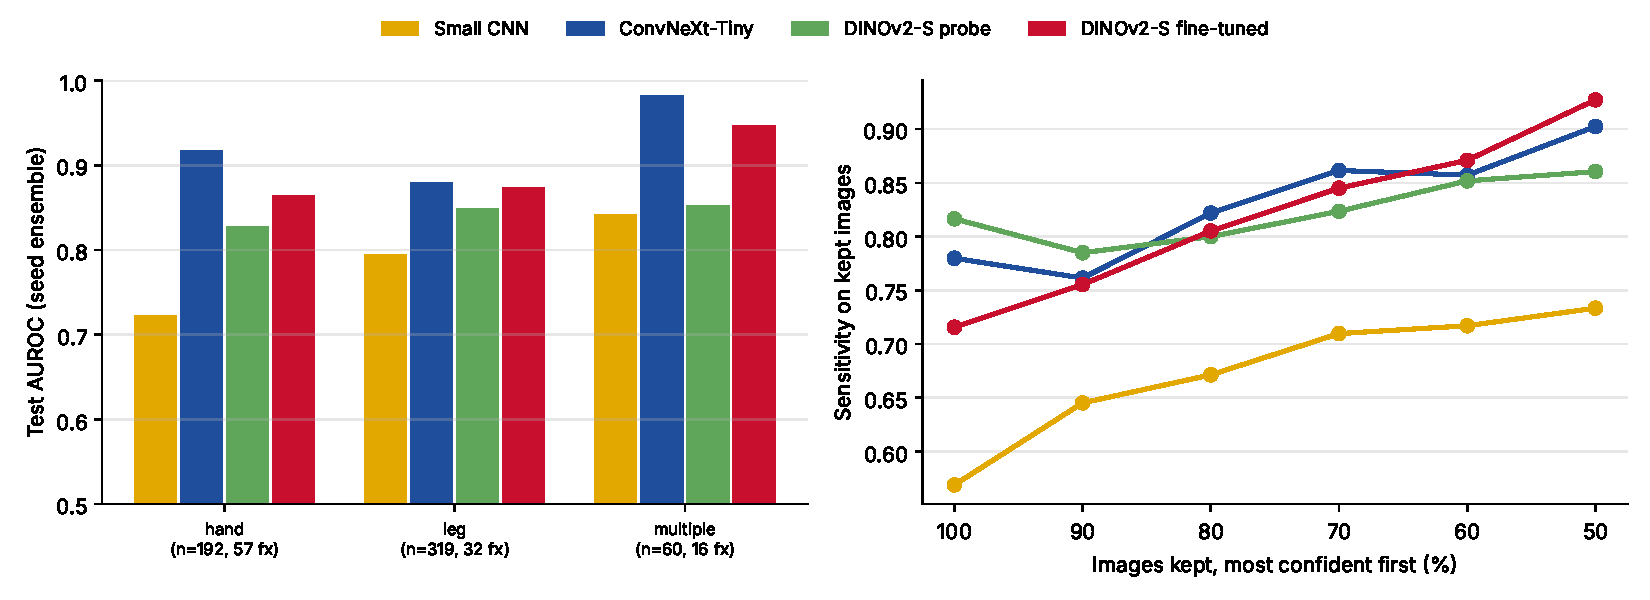
\includegraphics[width=\linewidth]{figures/fig_region_referral.pdf}
\caption{Left: test AUROC of the seed ensembles for the three regions with at least 16 fractured test images.
Right: sensitivity on the images a model keeps when it refers its least confident images (calibrated confidence
$\max(p,1-p)$; validation threshold).}
\label{fig:region}
\end{figure}

\paragraph{Operating point.} Table~\ref{tab:op} shows what the models do at a fixed threshold. ConvNeXt-Tiny has
the best average precision (0.835) and, at its validation threshold, finds 78\% of fractured images with 93\%
specificity (85 true and 34 false positives, 24 missed fractures). The frozen probe's threshold lands at a higher
sensitivity (0.82) but at the cost of 103 false positives against ConvNeXt's 34. Requiring 90\% sensitivity, ConvNeXt
keeps a specificity of 0.76; the other models fall to 0.45--0.66.

\paragraph{Where the models fail.} Table~\ref{tab:region} and Figure~\ref{fig:region} (left) break the results down
by body region. For every model, leg images are the weakest of the three well-populated groups: ConvNeXt reaches
AUROC 0.918 on hand images and 0.983 on multiple-region images but 0.880 on leg images, and at the shared threshold
it finds only 17 of 32 leg fractures (sensitivity 0.53, against 0.88 for hands). Leg images make up 15 of its 24
missed fractures. One likely contributor is prevalence: leg images have the lowest fracture rate (10\% of test leg images, against
30\% of hand images), so one threshold fitted on all regions is too high for them. Region-specific thresholds would raise leg sensitivity at the cost of more false positives;
we do not tune them here because the validation set has only 32 fractured leg images. The two fractured hip and two
fractured shoulder test images are all detected by ConvNeXt, but two images are no evidence either way.

\paragraph{Referral.} Figure~\ref{fig:region} (right) and Table~\ref{tab:referral} show what happens when a model
refers its least confident images. For ConvNeXt, keeping the most confident 80\% raises accuracy on the kept images
from 0.906 to 0.961 and specificity from 0.93 to 0.99, and sensitivity from 0.78 to 0.82; keeping half gives accuracy
0.984 and sensitivity 0.90. Most of the gain is in specificity: the uncertain images it refers are mostly false
alarms, while many of its missed fractures (in particular on leg images) are made with high confidence and are not
caught by referral. At 90\% coverage ConvNeXt's sensitivity even dips slightly (0.78 to 0.76), because the referred
tenth contains relatively more correctly detected fractures than missed ones. Its area under the risk--coverage
curve (0.024) is about half that of fine-tuned DINOv2 (0.045) and a quarter of the small CNN's (0.102). With a fixed
cut-off of 0.8 on the calibrated confidence, ConvNeXt refers 10\% of test images, fine-tuned DINOv2 25\%, the probe
36\% and the small CNN 45\%: a weaker model is not only less accurate but also much less often sure.

\begin{table}[t]
\centering
\caption{Sensitivity / accuracy on the kept test images when the least confident images are referred
(seed ensembles, calibrated confidence, validation threshold).}
\label{tab:referral}
\small
\setlength{\tabcolsep}{4pt}
\begin{tabular}{lcccccc}
\toprule
Kept & 100\% & 90\% & 80\% & 70\% & 60\% & 50\% \\
\midrule
Small CNN & 0.57 / 0.80 & 0.65 / 0.81 & 0.67 / 0.84 & 0.71 / 0.87 & 0.72 / 0.89 & 0.73 / 0.92 \\
ConvNeXt-Tiny & 0.78 / 0.91 & 0.76 / 0.95 & 0.82 / 0.96 & 0.86 / 0.97 & 0.86 / 0.98 & 0.90 / 0.98 \\
DINOv2-S probe & 0.82 / 0.80 & 0.78 / 0.86 & 0.80 / 0.89 & 0.82 / 0.91 & 0.85 / 0.93 & 0.86 / 0.94 \\
DINOv2-S fine-tuned & 0.72 / 0.88 & 0.76 / 0.90 & 0.81 / 0.92 & 0.85 / 0.94 & 0.87 / 0.95 & 0.93 / 0.97 \\
\bottomrule
\end{tabular}
\end{table}

\paragraph{Calibration.} Before scaling, the small CNN is badly calibrated (ECE 0.182) and the DINOv2 probe moderately
(0.139); ConvNeXt is already reasonable (0.057). Temperature scaling fitted on validation data lowers the ensembles' ECE for every
model, to 0.036 for ConvNeXt, but cannot fix a weak ranking: the small CNN remains at 0.151 after scaling, because many
of its test probabilities sit in the uncertain middle. For single seeds the picture is similar (ConvNeXt 0.066 to
0.042 on average), except for fine-tuned DINOv2, whose mean single-seed ECE does not improve (0.150 to 0.152): a
temperature fitted on validation data does not carry over to the test set for its less stable seeds.

\paragraph{Detector.} YOLO11s reaches box precision 0.438, recall 0.346, mAP@0.5 0.321 and mAP@0.5:0.95 0.143 on the
test images. This is lower than the 0.562 reported in the dataset paper, but the two numbers are not comparable: that
figure was measured on a validation set of fractured images only, while our test set contains more than four
non-fractured images for every fractured one, each a chance for a false box. (The Ultralytics validator read 606 of the
614 test images and their 133 fracture boxes.) Used as an image classifier through its highest box
confidence, the detector reaches AUROC 0.882 and finds 75\% of fractured images at 90\% specificity: better than the
small CNN and the frozen probe, but below ConvNeXt. A practical system can therefore use the classifier to decide
whether an image is likely to show a fracture and the detector to point to where.

\paragraph{Duplicates between splits.} FracAtlas contains exact copies of the same radiograph under different file
names: 20 test images and 23 validation images have a training image at Hamming distance 0, and 54 test images one
within 4 bits (Table~\ref{tab:dup}). Visual inspection of the closest pairs confirms that the distance-0 pairs are
the same image, and at least one of them carries opposite labels (IMG0004341, not fractured, in test; IMG0003034,
fractured, in training). Removing them barely moves the results: ConvNeXt's ensemble AUROC goes from 0.928 to 0.926
without exact copies and to 0.924 without copies within 4 bits, and the ranking of the four models is unchanged.
Larger thresholds remove many images that are only similar radiographs (the median distance to the nearest training
image is 10 bits), so we treat them as a stress test rather than as duplicate removal; even keeping only the 190 test
images farthest from any training image, ConvNeXt stays at 0.929 [0.870, 0.970]. Near-copies are therefore not what
drives the scores, although leakage between different images of one patient remains possible.

\begin{table}[t]
\centering
\caption{Test AUROC of the seed ensembles after removing test images whose nearest training image (perceptual hash)
lies within $d$ bits. Images (fractured) remaining in the second column.}
\label{tab:dup}
\small
\setlength{\tabcolsep}{4pt}
\begin{tabular}{lccccc}
\toprule
Removed & Test images & Small CNN & ConvNeXt-Tiny & DINOv2-S probe & DINOv2-S fine-tuned \\
\midrule
none            & 614 (109) & 0.809 & 0.928 & 0.873 & 0.902 \\
$d = 0$         & 594 (105) & 0.806 & 0.926 & 0.869 & 0.899 \\
$d \le 4$       & 560 (103) & 0.803 & 0.924 & 0.865 & 0.896 \\
$d \le 8$       & 389 (75)  & 0.807 & 0.927 & 0.873 & 0.903 \\
$d \le 12$      & 190 (42)  & 0.812 & 0.929 & 0.856 & 0.914 \\
\bottomrule
\end{tabular}
\end{table}

\section{Limitations}

FracAtlas releases no patient identifiers, so images of the same patient may fall into both training and test sets;
this can inflate test scores and is the most important caveat of every FracAtlas result, including ours. Our
hash check rules out exact and near copies as the source of the scores, but not different images of one patient.
The dataset also contains duplicated radiographs, some with conflicting labels, which any FracAtlas split inherits. All images
come from three hospitals in one country, and there is no external test set, so the numbers do not transfer to other
hospitals, devices or populations without new testing. The test set holds only 109 fractured images, and the hip-only
and shoulder-only groups contain two fractured test images each, so per-region estimates are uncertain and for those
two regions uninformative. Labels are at image level for the
classifiers; we did not use the masks. Hyperparameters were fixed in advance and not tuned per model, which may
disadvantage DINOv2 fine-tuning in particular. The confidence score and the referral curves describe this test set
and are not a safety guarantee. The models are research artefacts, not medical devices, and must not be used for
patient care.

\section{Conclusion}

On a fixed, stratified FracAtlas split with three seeds and bootstrap intervals, an ImageNet-pretrained ConvNeXt-Tiny
is the best and most stable fracture classifier (AUROC 0.928), clearly ahead of a small CNN trained from scratch and
ahead of DINOv2, whose frozen features are strong but whose fine-tuning varies between seeds. Leg radiographs are
its weak point, with half of the leg fractures missed at a shared threshold. After temperature scaling, ConvNeXt is
well calibrated and would refer only one image in ten at a confidence cut-off of 0.8; referral mainly removes false
alarms, so it does not replace a region-aware threshold for leg images. A YOLO11s
detector ranks images nearly as well but localises fractures only moderately. FracAtlas contains exact duplicates
across any image-level split, but removing them leaves the results unchanged. We suggest that future FracAtlas results
report several seeds, intervals, calibration and a referral curve, and state how the split was made.

\section*{Code and data availability}

Code, the Kaggle notebooks, per-seed logits and the analysis files are at
\url{https://github.com/MHKhan50/fracatlas-fracture-benchmark}, archived on Zenodo as version 0.2.0
(\href{https://doi.org/10.5281/zenodo.24429478}{doi:10.5281/zenodo.24429478}). A browser demo that runs both models
locally is at \url{https://huggingface.co/spaces/MHkhan50/fracture-xray-check}. The ConvNeXt-Tiny weights (seed 1, best validation
AUROC 0.941) with a model card are at \url{https://huggingface.co/MHkhan50/fracatlas-convnext-tiny}. FracAtlas is
available from figshare under CC BY 4.0 (\href{https://doi.org/10.6084/m9.figshare.22363012}{doi:10.6084/m9.figshare.22363012})
\citep{abedeen2023fracatlas}.

\bibliographystyle{plainnat}
\bibliography{references}

\end{document}
